	% -----------------------------------------------
% Styl pro psaní diplomových a bakalářských prací
% Určeno pro překlad pdfcsLaTeXem
% -----------------------------------------------
\documentclass[a4paper,12pt]{book} % pro oboustranný tisk zvolte {book}!
% velikost stránky
\usepackage[tmargin=2cm,bmargin=2.5cm,rmargin=2cm,lmargin=3.5cm]{geometry}
% volba kódování, nastaveno je unicode
\usepackage[utf8]{inputenc}
% \usepackage[cp1250]{inputenc}
% \usepackage[latin2]{inputenc}
\usepackage[english]{babel}
%\def\refname{Literatura}
% pomocná makra pro sazbu matematických výrazů
\usepackage{amssymb} %na psaní dvojitých písem a zvlastních znaků (např. \varkappa)
\usepackage{amsmath}
% balíček pro vkládání obrázků
\usepackage{graphicx}
% balíček pro obrázky na krajích stránky 
%\usepackage{floatflt}
% balíček pro křížové odkazy
\usepackage[unicode,bookmarksopen,colorlinks=false,plainpages=false,urlcolor=blue,pdfpagelabels]{hyperref}
% balíček pro vkládání hypertextových odkazů
\usepackage{url}

\usepackage{float}


\usepackage[numbers]{natbib}

% -----------------------------------------------
% Přepínač mezi bakalářskou a diplomovou prací, 
% barevným a černobílým logem a mezi studentem a studentkou (vypracoval/vypracovala apod.)
% -----------------------------------------------
\newif\ifbakal\bakaltrue
\newif\ifbarva\barvafalse
\newif\ifstudentka\studentkafalse

% -----------------------------------------------
% Údaje o práci – doplní se i do bibliografické identifikace, pouze v prohlášení je nutné vložit jméno vedoucího práce, které není v 1. pádě
% -----------------------------------------------
\newcommand{\nazevcz}{Kalibrace a monitorování astročásticových teleskopů}
\newcommand{\nazev}{Calibration and monitoring of astroparticle telescopes}
\newcommand{\student}{Daniel Staník}
\ifbakal%
  \newcommand{\program}{B0533A110007  Applied Physics}%
  \newcommand{\obor}{1702R001  Applied Physics  (AFYZ)}%
  %\else%
  %\newcommand{\program}{N1701 Fyzika}%
  %\newcommand{\obor}{7504T055 Učitelství fyziky pro střední školy}%
\fi
\newcommand{\rokod}{2022}
\newcommand{\vedouci}{Ing. Ladislav Chytka, Ph.D.}
\newcommand{\abstrakt}{%
Lorem ipsum dolor sit amet, consectetur adipiscing elit. Curabitur et lectus sit amet lectus vestibulum dignissim. Cras sit amet enim vitae mi elementum blandit eget nec tortor. Curabitur eget eros vitae arcu luctus varius commodo vel mauris. Nam elementum convallis pretium. Nunc dignissim pulvinar urna, nec blandit ante fringilla at. Ut et magna purus, vel pellentesque massa. In tortor nisi, faucibus condimentum cursus ut, sollicitudin quis leo. Ut at purus nec arcu accumsan tincidunt id id massa. Nam id vehicula mi.}
% -----------------------------------------------
\newcommand{\abstrakten}{%
Lorem ipsum dolor sit amet, consectetur adipiscing elit. Curabitur et lectus sit amet lectus vestibulum dignissim. Cras sit amet enim vitae mi elementum blandit eget nec tortor. Curabitur eget eros vitae arcu luctus varius commodo vel mauris. Nam elementum convallis pretium. Nunc dignissim pulvinar urna, nec blandit ante fringilla at. Ut et magna purus, vel pellentesque massa. In tortor nisi, faucibus condimentum cursus ut, sollicitudin quis leo. Ut at purus nec arcu accumsan tincidunt id id massa. Nam id vehicula mi.}
% klíčová slova
\newcommand{\klic}{klíčové slovo 1, klíčové slovo 2, \ldots}
\newcommand{\klicen}{keyword 1, keyword 2, \ldots}
\newcommand{\pocetstran}{xx}
\newcommand{\pocetpriloh}{x}

% -----------------------------------------------
% Definice vlastních maker pro usnadnění psaní
% a opakování symbolů při zlomu řádku
% -----------------------------------------------
% implikace se opakuje
\def\Plyne{\Rightarrow\discretionary{}{\hbox{$\Rightarrow$}}{}}
% -----------------------------------------------
% ekvivalence se opakuje
\def\Ekviv{\Leftrightarrow\discretionary{}{\hbox{$\Leftrightarrow$}}{}}
% -----------------------------------------------
% % plus '+' se opakuje při zalomení řádku
\mathchardef\plus="202B
\mathcode`\+="8000
{\catcode`\+=\active
\gdef+{\plus\nobreak\discretionary{}{\hbox{$\plus$}}{}}}
% opakování - při zalomení řádku
\newsavebox{\minusbox}
\savebox{\minusbox}{\hbox{$-$}}
\def\aktivniminus #1{{\catcode`#1=13 \bgroup \uccode`~=`#1
\uppercase{\egroup\gdef~}{\mathminus\discretionary{}{\copy\minusbox}{}}}}
% % -----------------------------------------------
% % rovnitko '=' se opakuje
\def\aktivnirovnitko #1{{\catcode`#1=13 \bgroup \uccode`~=`#1
\uppercase{\egroup\gdef~}{\mathequal\discretionary{}{=}{}}}}
% -----------------------------------------------
% zrušení mezery za čárkou v matematickém reľimu
\mathcode`,="002C

% -----------------------------------------------
% Úprava matematické sazby
% -----------------------------------------------
\def\sgn{\mathop{\rm sgn}\nolimits}
\def\tg{\mathop{\rm tg}\nolimits}
\def\cotg{\mathop{\rm cotg}\nolimits}
\def\arctg{\mathop{\rm arctg}\nolimits}
% -----------------------------------------------
% vektory polotučným skloněným písmem
\DeclareFontFamily{OT1}{bssbf}{}
\DeclareFontShape{OT1}{bssbf}{m}{n}{<5> <6> <7> <8> <9> <10> <11> <12> <14.4> <17> <20> <20.74> <25> bssb10}{}
\newcommand{\vek}{\fontencoding{OT1}\fontfamily{bssbf}\selectfont}
\renewcommand{\vec}[1]{\hbox{\vek #1}\hspace*{1.5pt}}
% polotučná řecká písmena
\def\bgomega{\vec{\char151}}
     \def\bgOmega{\vec{\char10}}
     \def\bggamma{\vec{\char130}}
     \def\bgvarphi{\vec{\char161}}
     \def\bgphi{\vec{\char148}}
     \def\bgxi{\vec{\char142}}
     \def\bgtau{\vec{\char146}}
     \def\bgeta{\vec{\char134}}
     \def\bgmu{\vec{\char139}}
     \def\bgnu{\vec{\char140}}
     \def\bvarrho{\vec{\char157}}
     \def\bgsigma{\vec{\char145}}
     \def\bgpsi{\vec{\char150}}
     \def\bgchi{\vec{\char149}}
     \def\bgvartheta{\vec{\char154}}

% ---------------------------------------------------------------
% Samotná práce
% ---------------------------------------------------------------
\begin{document}
% -----------------------------------------------
% Titulní strana
% -----------------------------------------------
\pagestyle{empty}
\setbox0=\hbox{\LARGE\scshape Joint Laboratory of Optics}
\centerline{\LARGE\scshape  Palacký University Olomouc}

\bigskip
\centerline{\LARGE\scshape Faculty of Science}
   
\bigskip
\centerline{\box0}
  
\vfill
\centerline{\LARGE\bfseries \ifbakal{BACHELOR}\else{DIPLOMOVÁ}\fi\ THESIS}

\bigskip
\begin{center}
{\huge\nazev}  


\vfill
\ifbarva
\includegraphics[height=3cm]{up_logo_color}\else%

\includegraphics[height=3cm]{up_logo_bw}\fi

\vfill

\noindent%
\begin{tabular}{ll}
Author\ifstudentka{a}\fi: & {\bfseries\student}\\
Study program: &\program\\
Field of study: &\obor\\
Form of study:& Full-time\\
Supervisor:& \vedouci\\
Deadline:& April~\rokod
\end{tabular}
\end{center}

% ---------------------------------------------------------------
% Prohlášení
% -----------------------------------------------
\newpage
\hbox{~}

\vfill

\begin{center}
{\bf DECLARATION}
\end{center}

\noindent
I hereby declare that I elaborated this bachelor thesis independently under the supervision 
of  Ing. Ladislav Chytka, Ph.D.,  using  only  information  sources  referred  in  the  Literature chapter. \\
{}\vspace{3ex}

\noindent
In~Olomouc~\today   \hfill\parbox[t]{6cm}{\centering\null\dotfill\\\student}

% -----------------------------------------------
% Bibliografická anotace
% -----------------------------------------------
\newpage
% Bibliografická identifikace
\section*{Bibliographical identification}

\begin{tabular}{lp{8cm}}
%-----------
% \multicolumn{2}{c}{\bfseries Bibliographical identification}\\[8mm]
%-----------
Autor's first name and surname & \student\\
%-----------
Title & \nazev\\
%-----------
Type of thesis & \ifbakal{Bachelor}\else{Master}\fi \\
%-----------
Department & Joint Laboratory of Optics \\
%-----------
Supervisor & \vedouci\\
%-----------
The year of presentation & \rokod \\
%-----------
Abstract & \abstrakten\\
%-----------
Keywords & \klicen\\
%-----------
Number of pages & \pocetstran\\
%-----------
Number of appendices &  \pocetpriloh\\
%-----------
Language & czech\\
%-----------
\end{tabular}

% -----------------------------------------------

\newpage
\section*{Bibliografická identifikace}

\begin{tabular}{lp{8.5cm}}
%-----------
% \multicolumn{2}{c}{\bfseries Bibliografická identifikace}\\[8mm]
%-----------
Jméno a příjmení autora & \student\\
%-----------
Název práce & \nazevcz \\
%-----------
Typ práce & \ifbakal{Bakalářská}\else{Diplomová}\fi \\
%-----------
Pracoviště & Společná Laboratoř Optiky \\
%-----------
Vedoucí práce & \vedouci\\
%-----------
Rok obhajoby práce & \rokod\\
%-----------
Abstrakt & \abstrakt\\
%-----------
Klíčová slova & \klic\\
%-----------
Počet stran & \pocetstran\\
%-----------
Počet příloh & \pocetpriloh\\
%-----------
Jazyk & český\\
%-----------
\end{tabular}
% %%%%%%%%%%%%%%%%%%%%%%%% End of file %%%%%%%%%%%%%%%%%%%%%%%%





%%%% Tady začínáme %%%%%%%%%%%%%%%%%%%%%%%%%%%%%%%%%%%%%%%%%%%%%%%%%%%%%%%%%%
\newpage
%%%%%%%%%%%%%%%%%%%%%%%%%%%%%%%%%%%%%%%%%%%%%%%%%%%%%%%%%%%%%%%%%%%%%%%%%%%%%
\widowpenalty =10000
\pagestyle{plain}
% -----------------------------------------------
% Obsah je generován automaticky, změny se projeví po 2 překladech
% -----------------------------------------------
\tableofcontents

% -----------------------------------------------
% Úvod
% -----------------------------------------------
\chapter*{Introduction}
\addcontentsline{toc}{chapter}{Introduction}

Lorem ipsum dolor sit amet, consectetur adipiscing elit. Curabitur et lectus sit amet lectus vestibulum dignissim. Cras sit amet enim vitae mi elementum blandit eget nec tortor. Curabitur eget eros vitae arcu luctus varius commodo vel mauris. Nam elementum convallis pretium. Nunc dignissim pulvinar urna, nec blandit ante fringilla at. Ut et magna purus, vel pellentesque massa. In tortor nisi, faucibus condimentum cursus ut, sollicitudin quis leo. Ut at purus nec arcu accumsan tincidunt id id massa. Nam id vehicula mi. 

\url{http://exfyz.upol.cz/didaktika/}

% -----------------------------------------------
% Kapitoly lze ukládat do zvláštních souborů...
% -----------------------------------------------
% -----------------------------------------------
% Vlastní text práce (kapitoly práce)
% -----------------------------------------------

% -----------------------------------------------
\chapter{Astroparticle detection}
% -----------------------------------------------
More than 100 years have passed since Victor Franz Hess first encontered cosmic radiation. Since those times the techniques and methods of detection have been strongly improved. We have moved up from elevating electroscopes by ballons to observe growing electric charge to specialized techniques, which allows us to measure particles' energies, trajectories, etc.

% -----------------------------------------------
\section{Cosmic rays and particles}
% -----------------------------------------------
Cosmic rays is a term for radiation and energetic particles striking earth atmosphere with an origin in a space sources (neutron stars, supernovas, black holes, etc). We divide them into two major groups - primary and secondary. Primary cosmic rays are the original cosmic particles, which strike the Earth's athmosphere. Secondary cosmic rays (also refered as showers) are particles, which have origin in particle interaction between primary cosmic rays and the athmosphere.
\par
\subsection{Primary cosmic rays}
Primary cosmic rays consist of protons ($95 \%$), helium nuclei ($4 \%$), electrons and other heavy nuclei (up to iron). However, only the energetic rays make their way to the athmosphere. The Earth's magnetic field affects their trajectories and prevents the low-energetic (less than 100 MeV) particles from arriving to the athmosphere \cite{Kliewer}. 
\par
Part of primary cosmic rays are also Ultra-high energy cosmic rays (UHECRs), which we refer in the next chapter.
\par 
Neutrinos are also a part of cosmic radiation, but their interaction with matter is very rare, so they are very hard to detect. The special underwater detectors are developed to detect some of them. 
\subsection{Secondary cosmic rays}
Secondary cosmic rays are created by interaction of high-energetic particles of primary component with air's nucleis, such as nitrogen. They consist of low-energetic and high-energetic muons, gamma photons, electrons and positrons. Most of muons travel up to the earth's surface although their half-life is only about 2.2 microseconds before they decay into electrons. Due to their high relativistic speeds, their half-life is increased for external observers. 




% -----------------------------------------------
\section{Ultra-high energy cosmic rays (UHECRs)}
UHECRs are particles with energies from $10^{18}$ to $10^{20}$ eV, which is much more than particles created on Cern's Large hadron colider (LHC) with energies about $10^{13}$. Due to their high energies, the trajectory remains nearly unchanged by space magnetic fields \cite{Benjamin_Skuse}.
\par
UHECRs' origin is yet unknown, but it is supposed and experimentally proved that they come from outside of the Milky Way. Some theoretical physicists expects, that the one possible source of UHECRs acceleration are the starburst galaxies.
\par
When the UHECR interacts with athmospheric nuclei,

% -----------------------------------------------
\section{UHECRs detection techniques}


\subsection{Pierre Auger observatory}
% -----------------------------------------------

\subsection{Telescope array project}
% -----------------------------------------------
% %%%%%%%%%%%%%%%%%%%%%%%% End of file %%%%%%%%%%%%%%%%%%%%%%%%

% -----------------------------------------------
% -----------------------------------------------
% Vlastní text práce (kapitoly práce)
% -----------------------------------------------

% -----------------------------------------------
\chapter{FAST telescope}
% -----------------------------------------------
The  Fluorescence  detector  Array  of  Single-pixel  Telescopes  (FAST) is an international project of fluorescence telescope sensitive to UHERCs. 
\par
Until today there are four prototypes in active service. Three of them are situated in Black Rock Mesa site of the Telescope Array experiment in central Utah and one in Argentina near Pierre Auger Observatory.
\par
The main goal of FAST project is to develop a cheap fluorescence telescope, which could be used in future to cover the wide surface area. This new oncoming fluorescence telescope array should be able  
to fully reconstruct the geometry of UHERCs induced UV shover by combining the information from telescopes, which has encountered some event at the same time. 
% -----------------------------------------------
\section{Principle of operation}
% -----------------------------------------------
Main detection part of telescope consists of superreflective UV mirrors and photomultipliers. 


\par
The entire telescope along with monitoring systems and other instruments is situated in a hut with remote shutter, where it is protected from negative metrological phenomena, such as rain or fast wind, but also from dust and aerosols. Exposure of mirrors to any of this phenomena could lead to reduction of theirs reflectivity. It is also neccessary to monitor and protect PMTs from unwanted light sources. Even a low-intensity sources could decrease PMT's service life.
% -----------------------------------------------

\section{Remote control and monitoring}
% -----------------------------------------------

%------------------------------------------------

\section{}
% -----------------------------------------------



% -----------------------------------------------
% %%%%%%%%%%%%%%%%%%%%%%%% End of file %%%%%%%%%%%%%%%%%%%%%%%%

% -----------------------------------------------
% -----------------------------------------------
% Vlastní text práce (kapitoly práce)
% -----------------------------------------------

% -----------------------------------------------
\chapter{Instrumentation}
% -----------------------------------------------
To perform all of necessary measurements we need to use various types of optical and electronic equipment, which is discussed in this chapter.
% -----------------------------------------------
\section{Integration sphere}
% -----------------------------------------------
The Integration sphere (IS) is a special optical equipment, which can be used either as extended uniform light source (EULS) e.g. with spectrometer in determining the material reflectance. In our experiments we use general purpose Labsphere (Fig. \ref{Labsphere}).

\begin{figure}[H]
 \centering
 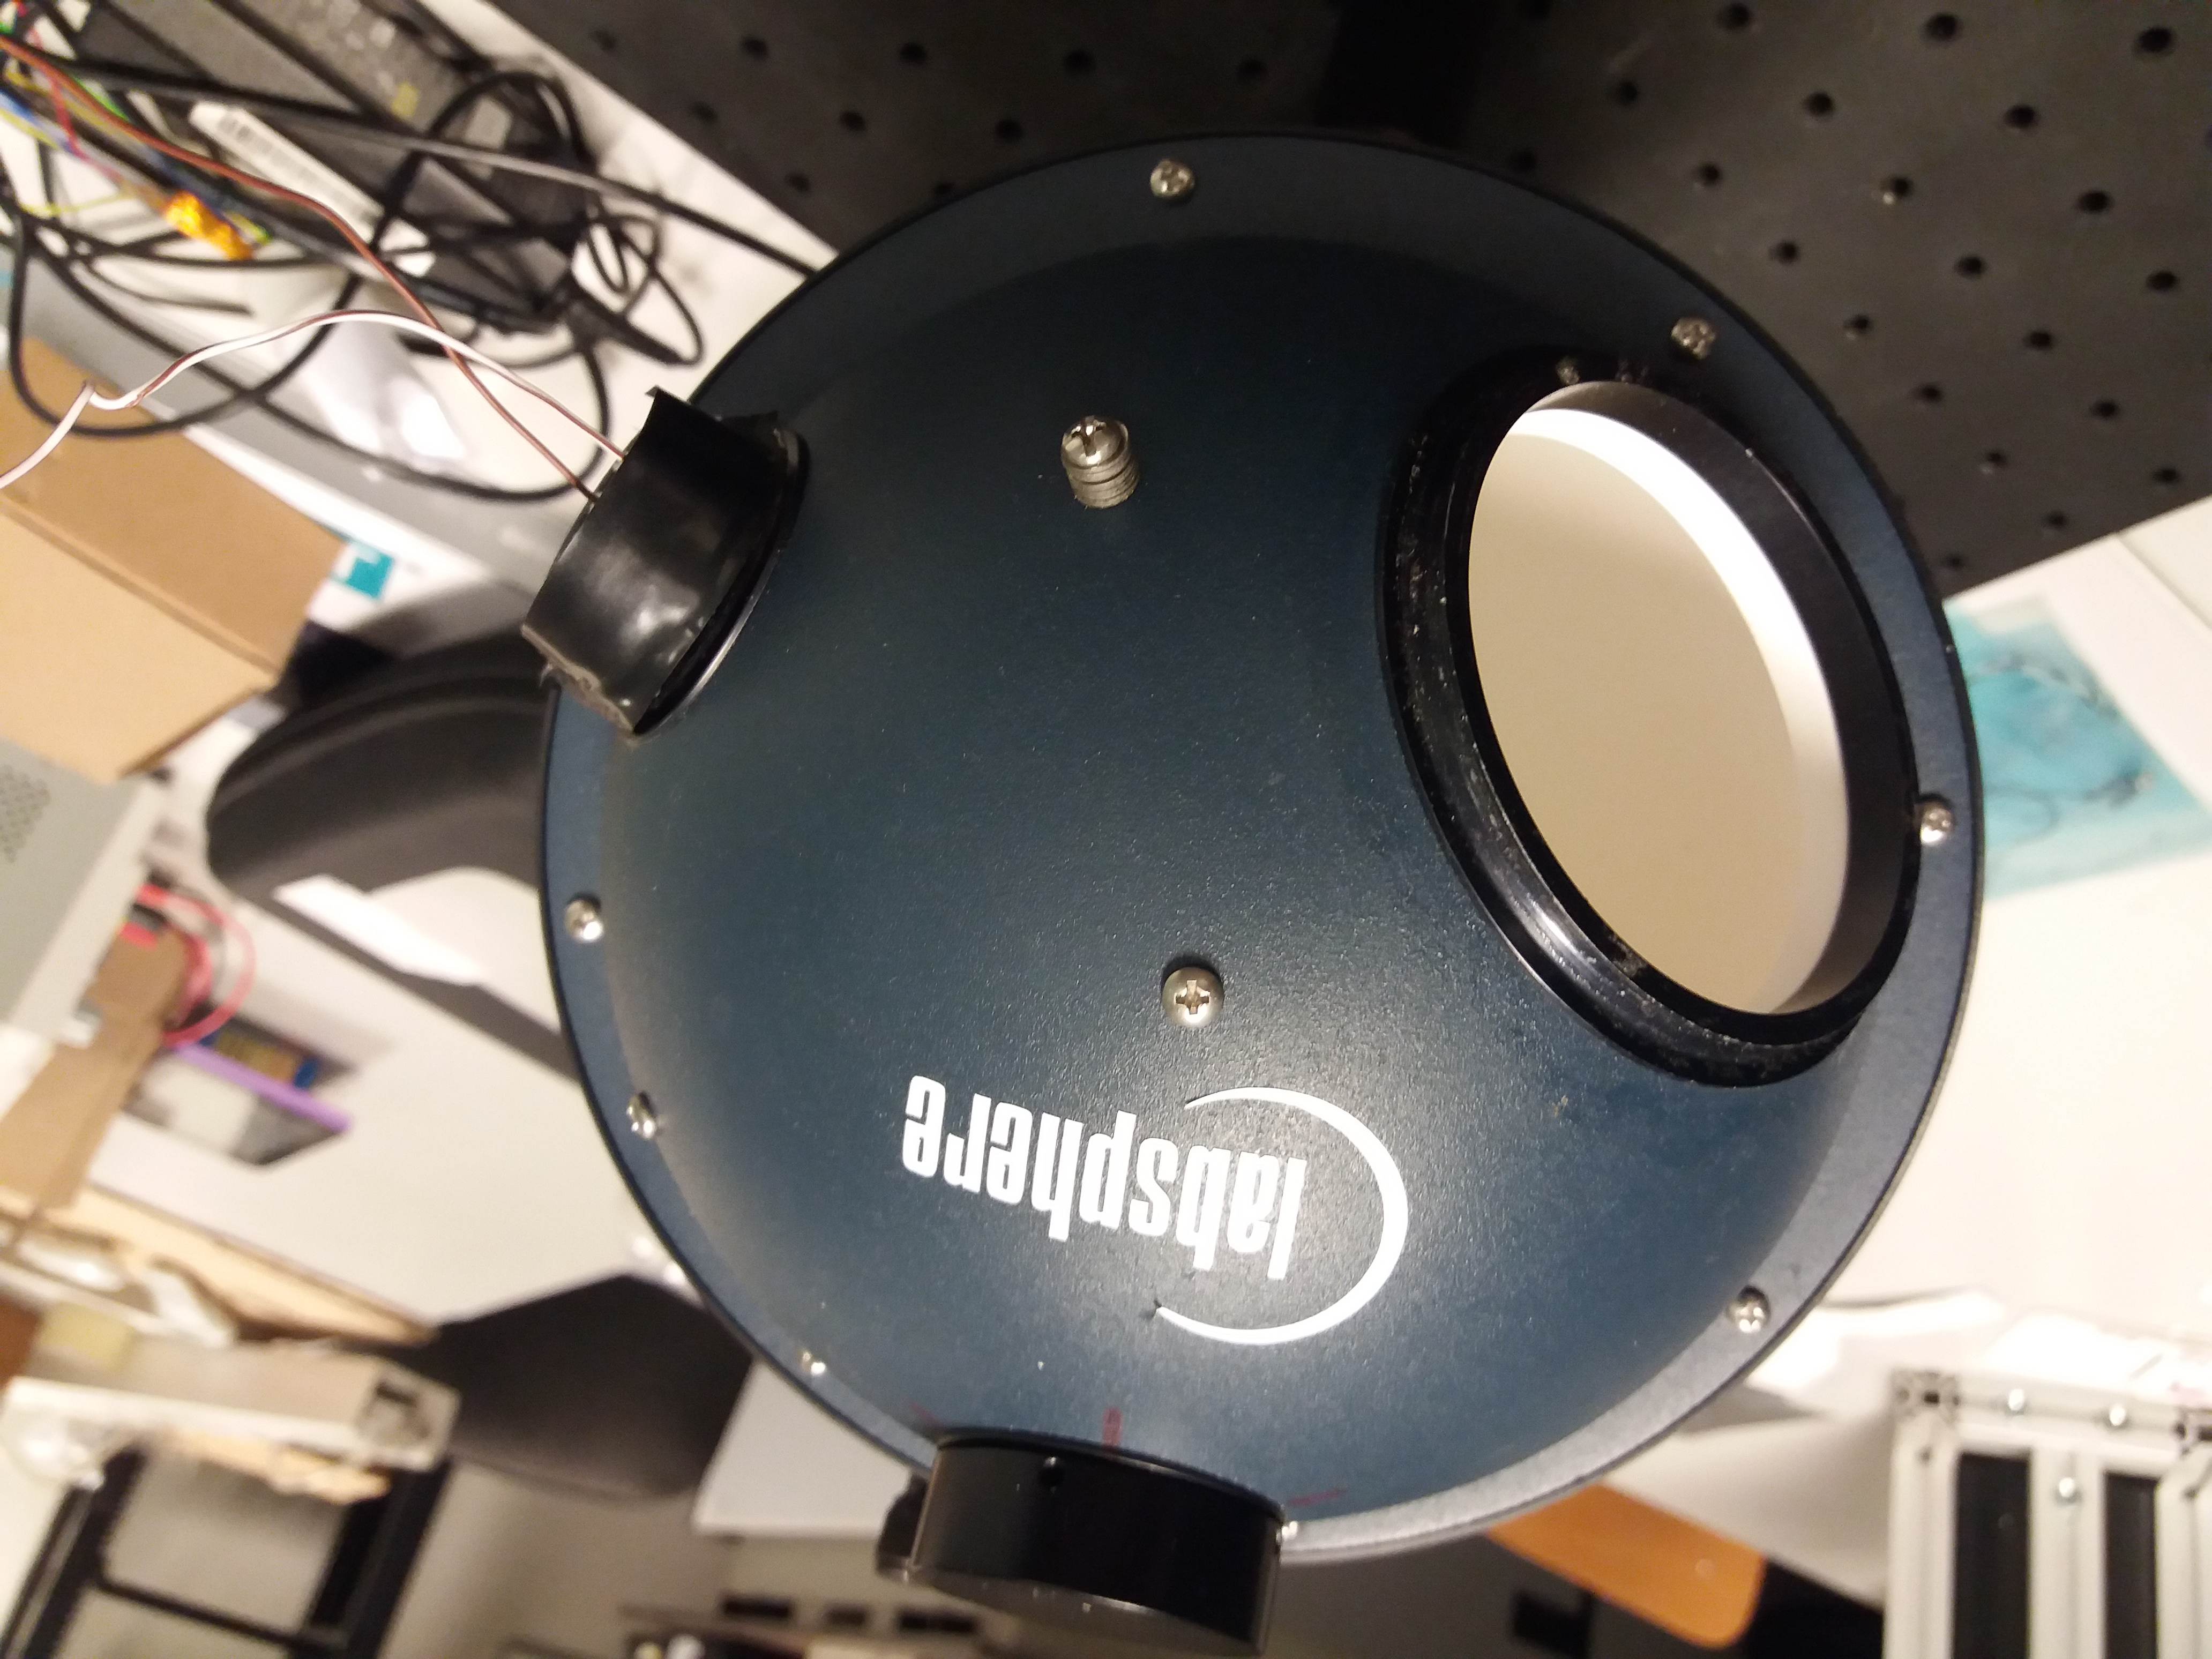
\includegraphics[scale=0.09, angle = 180]{./pictures/IntegrationSphere}
 \caption{General purpose Labsphere.}
 \label{Labsphere}
 
\end{figure}
\par
The IS inner surface consist of white optical diffusive material (BaSO$_4$ and Polytetrafluoroethylene). The IS also contains several circular apertures, which are called input/output ports. These can be used to mount detectors or optical sources or left free to let light flux enter or exit IS. 
\par
The inner surface is the part where light integration happens. The effect which takes place here is known as Lambertian scattering. After one spot of inner surface is hit by a ray, the energy should be uniformly radially distributed. In output port this produces a homogeneous light source. The homogeneity decreases with increasing number and sizes of input/output ports.
\par
Using optical source with IS typically requires baffle to prevent source's light flux or its part to exit IS without integration.
\par
Deep explanation of IS working principles and characterization of optical properties of the identical IS, which we use, can be found in \cite{VACULA2021167169}.
\par
For our purposes, in case of FAST calibration, we use IS as an UV EULS. In case of testing optical UV calibration source, we use IS mainly to block the possible incoming external light and to distribute the optical power of the UV source between mounted detectors.
% -----------------------------------------------

\section{Photomultiplier tube}
% -----------------------------------------------
Photomultiplier tube (PMT) is considered to be a high voltage optoelectronical part. It allows us to measure very low intesity optical signals. PMT is also characterized by high amplification, low noise and stability. It has many variants of usage. It can be used either as detector of optical signal (pulse or continual) for chosen wavelength or as a radiation detector. The general theory of PMTs is described in more detail in \cite{Photonis, Hamamatsu}. 
\subsection{Operating principle}
PMT consists of 6 main elements, which can be seen on scheme \ref{PMT scheme}.

\begin{figure}[H]
 \centering
 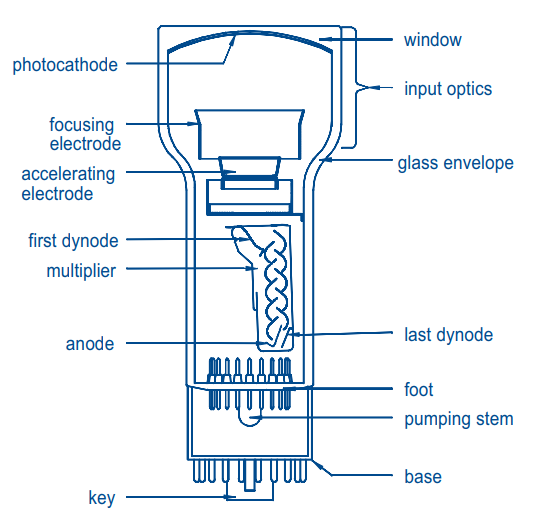
\includegraphics[scale = 0.5]{./pictures/PMTscheme}
 \caption{Photomultiplier tube scheme \cite{Photonis}.}
 \label{PMT scheme}
\end{figure}

\begin{figure}[H]
 \centering
 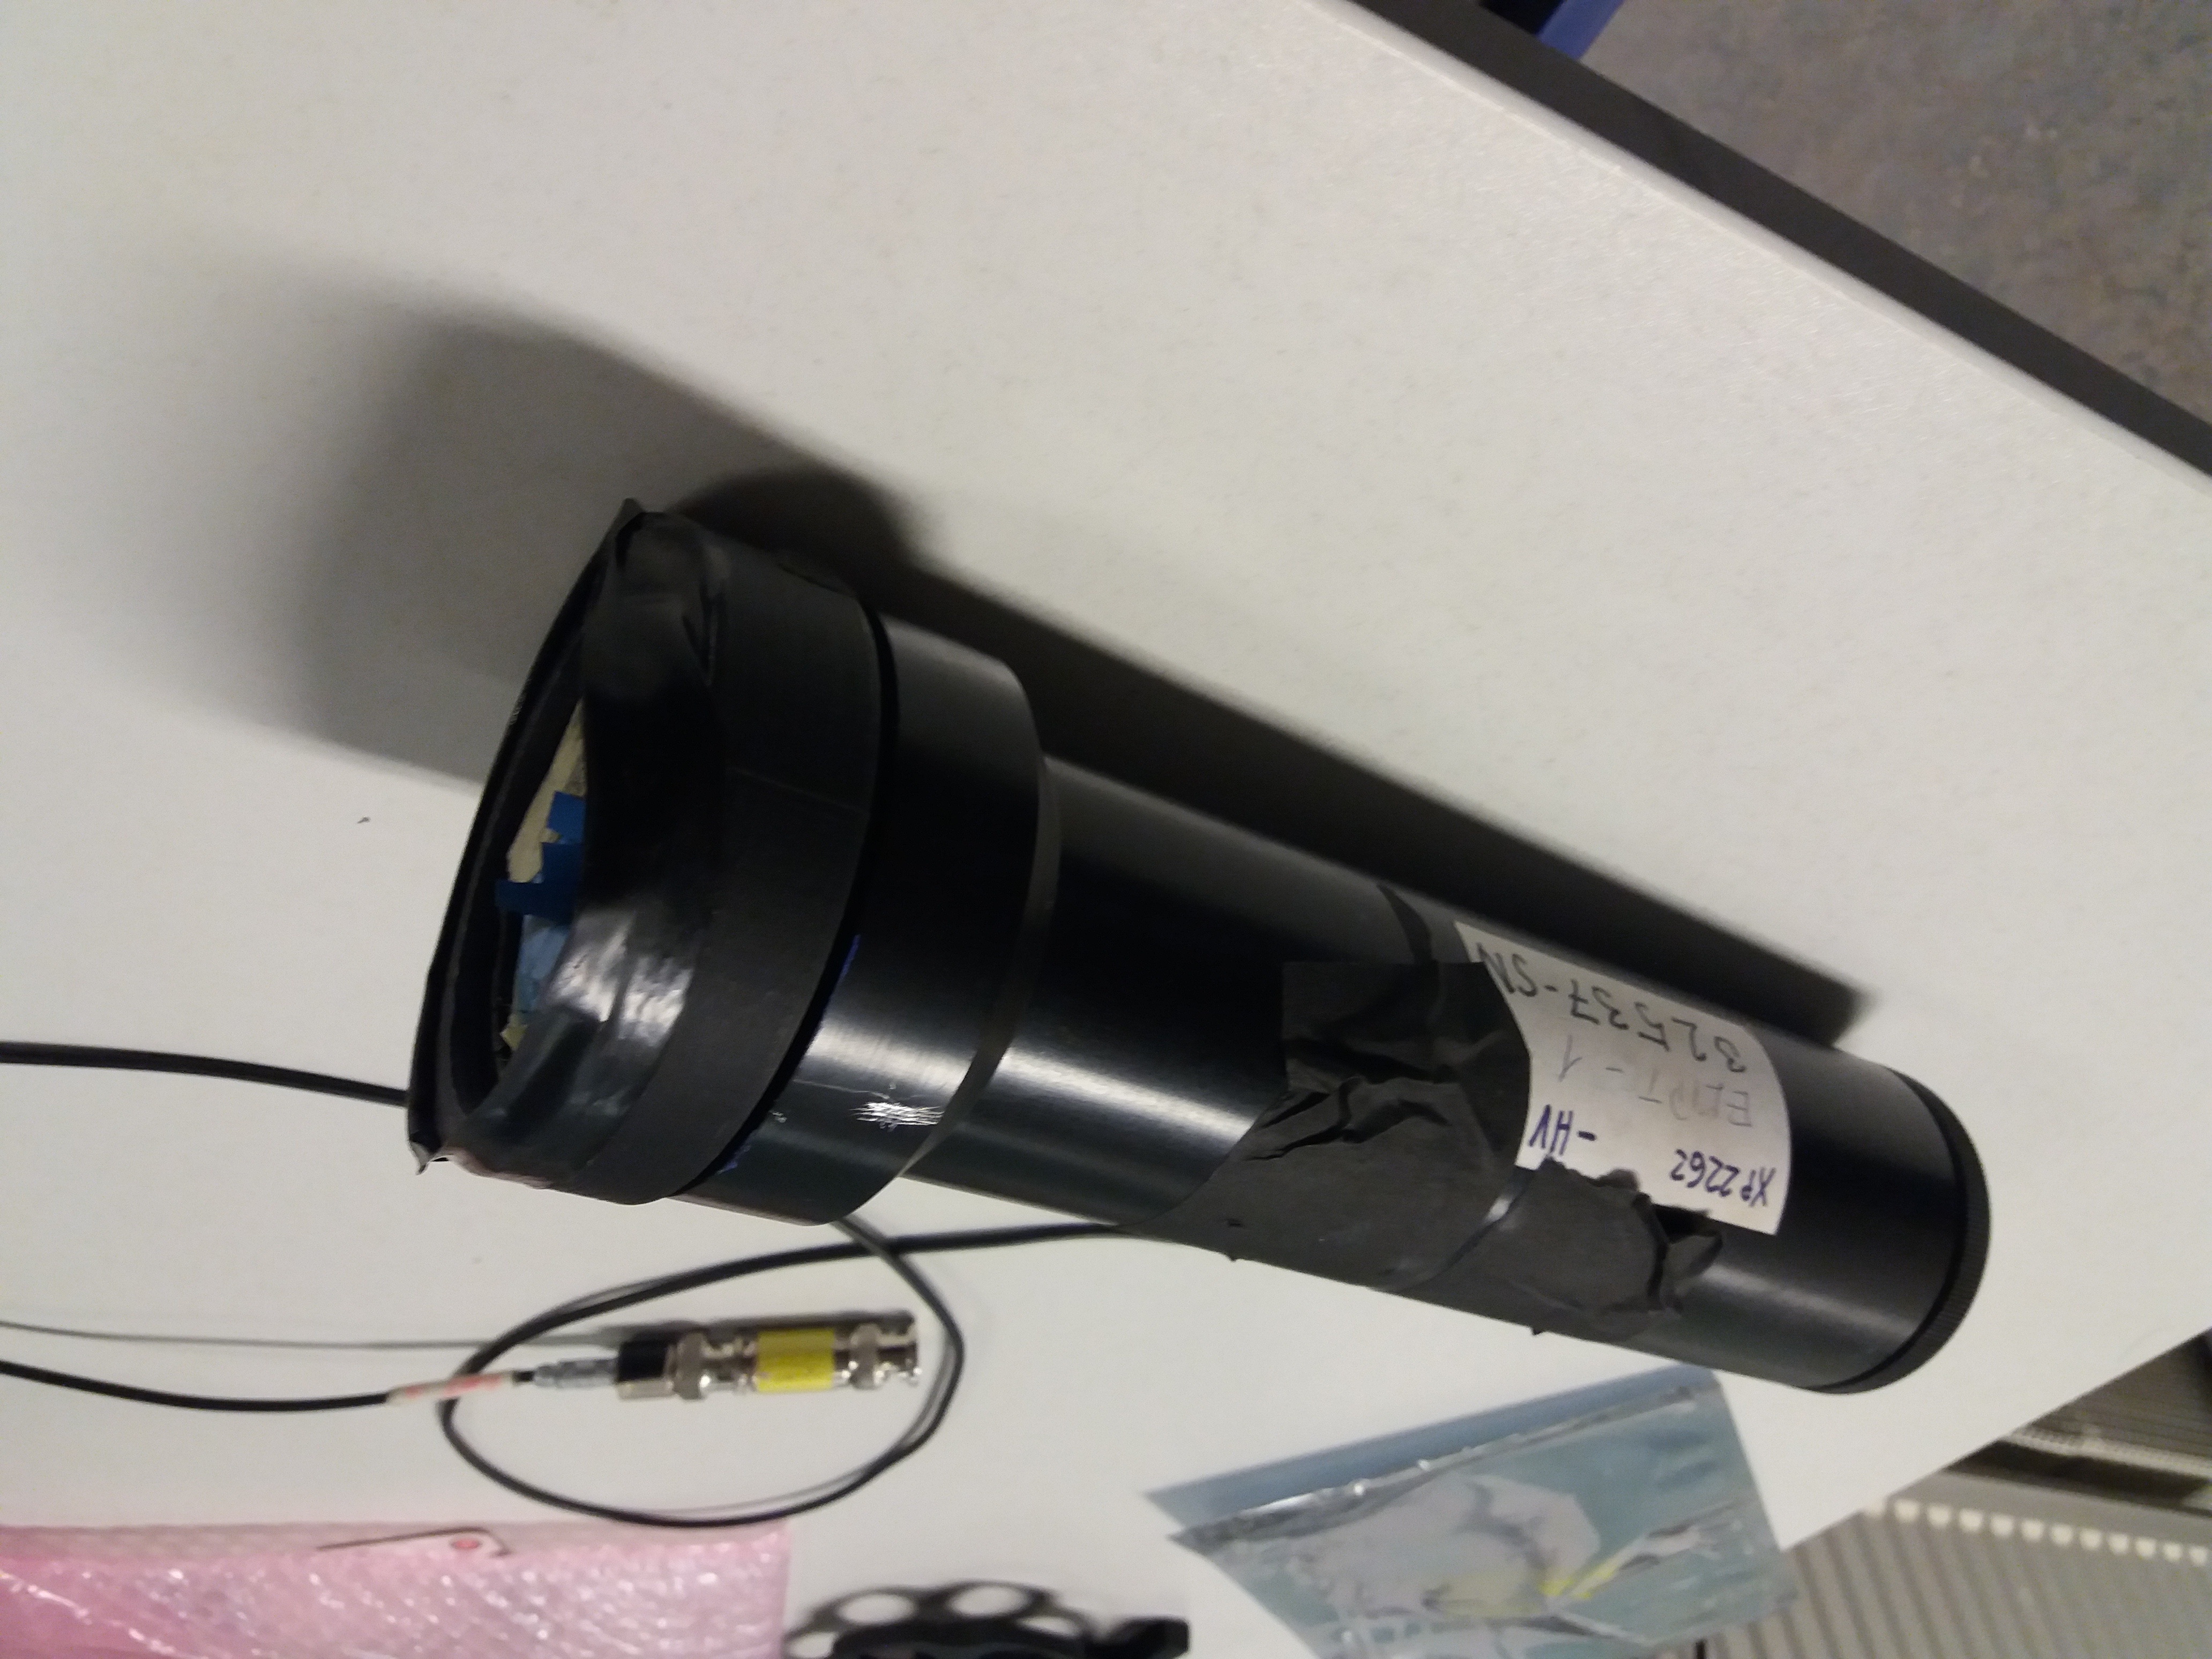
\includegraphics[scale = 0.08, angle = 180]{./pictures/XP2262}
 \caption{XP2262 PMT in a metal enclosure used for our measurements.}
 \label{XP2262 PMT}
\end{figure}

\par
The input photon with sufficient energy, which strikes the PMT's photocathode, excites photocathode's electron. This electron then follows electrostatic field to the first dynode of the electron multiplier, where it induces secondary emission of more electrons. These electrons are then attracted by the next dynode, where the emission process repeats. After few times of multiplying electron number over dynodes, the electrons are then collected by 
the anode, which is situated on the end of the electron multiplier. The anode output current is then converted to voltage signal by appropriate load resistor or by operational amplifier current-to-voltage circuit.
\par
As all other laboratory instruments, which are based on accelerating electrons, such as electron microscopes, the photomultiplier's main parts must be kept in vacuum. To maintain vacuum, the photomultiplier is surrounded by special glass envelope. To avoid mechanical damage of the glass envelope, the entire photomultiplier is sometimes situated in a plastic tube.
\par
One of the basic adjustable characteristics of PMT is its gain. The gain is defined as:

\begin{equation}
G = \frac{I_\textrm{a}}{I_\textrm{p}},
\end{equation}
where $I_\textrm{a}$ is the anode current and $I_\textrm{p}$ is the input photocurrent from the photocathode.
\par
In case of ideal, noiseless PMT, we can adjust gain by varying the supply voltage. By varying supply voltage we can adjust gain according to an equation:

\begin{equation}
\frac{G_2}{G_1} = (\frac{V_2}{V_1})^{\alpha N},
\label{gainVolt}
\end{equation}
where $G_2$ and $G_1$ are gains at supply voltages $V_2$ and $V_1$. $\alpha$ is coefficient given by dynode material and $N$ is the number of dynodes.
\par
Other effects, such as temperature, may also vary PMT's gain, and it is necessary to keep them on constant value or measure them and involve them in the final evaluation of data.
\par
For the proper functionality of the PMT, the charge and current linearity should be considered. Charge linearity is the ratio of the number of incident photons to the number of electrons collected at the anode. Current linearity expresses the proportionality between incident light flux and anode current. Ideal PMT is always linear, but the real PMT may vary from linearity due to drifts, space charges, instability of voltage divider etc. These effects can lead up to saturation of the PMT. In saturation, increasing the input light flux leaves the anode current mostly unchanged.      


\subsubsection{Window}

The photocathode is coated on glass window, whose main purpose is to admit light of certain wavelengths. Glass materials are characterized by the spectral sensitivity to wavelengths. For transparency in UV spectre, it is advised to use borosilicate or fused silica glasses.


\subsubsection{Photocathode}

The photocathode is the only light-sensitive part of PMT. It transfers the light flux into the electric current.
\par
One of its main parameters is quantum efficiency. It is referred to as ratio of emitted photoelectrons to the number of incident photons expressed as a percentage. It is generally less than 35 \%. For measurement, the more practical parameter is cathode radiant sensitivity. It is the ratio of photocathode current to an incident light power, which is expressed in mA/W.
\par
Photocathode material must be sensitive to certain wavelengths, which we want to detect with the PMT, and must have sufficient quantum efficiency. Preferred materials are usually alkali antinodes.
\subsubsection{Electron multiplier}
The electron multiplier consists of dynodes and one anode.
Dynodes are electrodes, which produce more electrons through secondary emission. To maintain electrostatic field between dynodes, each of dynodes is held on different potential. This is achieved by using the voltage divider. Every resistor in the divider sets the potential of one diode according to its resistivity.
\par
All of the photoelectrons emitted by photocathode should be ideally collected by the first dynode. However, many of them could be diverted from their path to dynode due to various effects. The parameter, which characterizes this, is the collection efficiency. The collection efficiency is probability that a photoelectron will strike area of the first dynode. 
\par
There are few types of dynodes arrangements. On the fig. \ref{PMT scheme} is the classic linear-focusing multiplier. 


\subsubsection{Voltage divider and voltage adjustment}
Voltage divider could be a simple resistor serial network, which divide high input voltage between the dynodes. 
\par
It is necessary to consider, that the multiplier current density increases in direction to the anode, so it tends to lessen the voltage between last dynode and anode. This phenomena can shake the potential levels across the entire multiplier. One way to reduce the impact on PMT's behaviour is to choose the proper resistor values of the divider. 
\par
The resistor values could same for all the dynodes, but for some applications it is better to have progressive voltage distribution, which increases from cathode to anode, or intermediate distribution with highest values on the beginning of the multiplier.

\par
In some applications, where high anode current peaks are expected, the divider can be filled with reservoir capacitors, which prevent the temporally charge exhaustion of the dynodes. In pulse mode, the unwanted oscillations on dynodes may occur, in that case, it is desirable to connect additional damping resistor to the divider.
\par
Voltage supply should be stable during the PMT's operation. As was mentioned before, the PMT's gain is voltage dependent. To adjust sufficient gain, high voltage (hundreds of volts) needs to be applied between photocathode and anode. The high voltage needs to be ramped on required level gradually to avoid negative consequences of transition and dark current effects, which can decrease the operating life of PMT. The same is valid for shutting down the PMT.
\par
The high voltage could be applied to the PMT in negative or positive polarity. In case of positive polarity, the cathode is held at ground and anode on +HV. In case of negative polarity, the cathode is held at -HV and anode at ground. 

\subsection{Dark current}
Dark current is the anode current produced by a photomultiplier in total darkness. It is considered to be a part of unwanted noise, causes errors in measurements and limits the detectivity of PMT. Dark current has origin in ohmical leakage, thermionic and field emission or in radioactivity. Ohmical leakage is major part of dark current at low gain. With the increasing gain the thermionic emission prevails. At high gains the field emission becomes the major part.
%\subsubsection{Ohmical leakage}
%Insufficent insulation of electrodes, dynodes and all other parts which are under high voltage may lead to surface current over glass and tube. Dirt and humidity are in most cases the reason of Ohmical leakage.

%\subsubsection{Thermionic emission}
%Temperature causes emission of photocathode's electrons, which are at medium gains the major part of dark current.  Due to this effect, some PMTs may need to be cooled during operation.
%\subsubsection{Field emission}
%At high gains the electrostatic field is so strong that it can rip the electrons out of the electrodes and accelerate them onto other surfaces, where they cause secondary emission. Field emission rapidly increases with supply voltage. In some literature it is also refered as cold emission.
%\subsubsection{Radioactivity}
%The radioactivity of PMT's components depends only on the material composition. In some aplications, such as astroparticle detection, it is neccessary to decrease radiation as possible. In astroparticle detection the radioactivity could be a source of false events. Only way to prevent this is to use materials with a very low concentration of radioactive isotopes.

\subsection{Timing and response}
Differences of photoelectrons' trajectories from the cathode to the first dynode lead into time distortion of signal. For example if we were able to produce delta-function pulse, the PMT would detect pulse with some response width time $t_\textrm{w}$.
With respect to differences in electron trajectories and arrival times, the PMTs are divided into 3 types:
\begin{enumerate}
\item \textbf{Very-fast tubes} - photoelectrons arrive simultaneously, low collection efficiency.
\item \textbf{Fast tubes} - compromise between timing performance and collection efficiency
\item \textbf{General-purpose tubes} - simple optoelectronics, good collection efficiency, low timing performance
\end{enumerate}
%\par 
%Another time delay to be considered 

\subsection{Operating life and degradation}
The operating life of PMT is defined as the time required for anode sensitivity to be halved. If we neglect the outside effects, the operating life mainly depends on anode current. 
Degradation processes start to show themselves at currents higher than 10 $\mu$A. Ageing is accompanied by increasing or decreasing gain at stable voltage. Operating life of PMT is measured in thousands of operating hours.
\par
By exposing PMT to bad conditions, such as humidity, mechanical stress, high temperatures or the high-intensity light, the PMT's operating life could be shorten much faster.
%------------------------------------------------
%------------------------------------------------

\section{Hardware for experiment control}
% -----------------------------------------------

\subsection{Raspberry Pi}
Raspberry Pi (RPi) is a single board computer which we use mainly for the experiment control. The linux-based Raspbian or DietPi operating system allows us to easily run various scripts and programs written in multiple languages. By having wifi and an ethernet port, the RPi can be easily accessed over internet. It can be used to control instruments and data acquisition over its USBs,1-Wire and I2C etc. However, it doesn't have any analog inputs/outputs such as ADCs and DACs.
\subsection{STM32 based microcontrolers}
For other types of tasks, which do not require data storage and remote control, but require for example an analog sampling, setting up the voltage levels or generating well defined PWM pulses, we use STM32 based microcontrollers. 
\par
For this thesis purposes we use the STM32 nucleo F411RE and the STM32 nucleo F446RE with better analog inputs/outputs.
% -----------------------------------------------
% %%%%%%%%%%%%%%%%%%%%%%%% End of file %%%%%%%%%%%%%%%%%%%%%%%%

% -----------------------------------------------
% Závěr
% -----------------------------------------------
\chapter*{Conclusion}
\addcontentsline{toc}{chapter}{Conclusion}

We are completely f****d.

% -----------------------------------------------
% Literatura a prameny
% -----------------------------------------------
%\begin{thebibliography}{99}
\bibliographystyle{apsrev4-2}
\nocite{*}
\bibliography{citations}
%\addcontentsline{toc}{chapter}{Literatura}
%\bibitem{gravitation} MISNER, Ch. W.; THORNE, K. S.; WHEELER, J. A. %\emph{Gravitation}. San Francisco: W. Freeman, 1973.
%\end{thebibliography}

\newpage
Preferované jsou citace podle norem ČSN ISO 690 a ISO 690-2, popř. styly APS (American Physical Society – u~prací zaměřených fyzikálně) nebo APA (American Psychological Association – u~prací zaměřených více didakticky a pedagogicky).
\end{document}
% Konec souboru %%%%%%%%%%%%%%%%%%%%%%%%%%%%%%%%%%%%%%%%%%%%%%%%%%%%%%%%%%%%
